\documentclass[border=2pt]{standalone}
\usepackage[T1]{fontenc}
\usepackage{lmodern}
\usepackage{amsmath,amssymb}
\usepackage{tikz}
\usepackage{pgfplots}
\pgfplotsset{compat=1.17}
\usepgfplotslibrary{groupplots}
\usetikzlibrary{arrows.meta,calc,positioning,fit,backgrounds}

\begin{document}
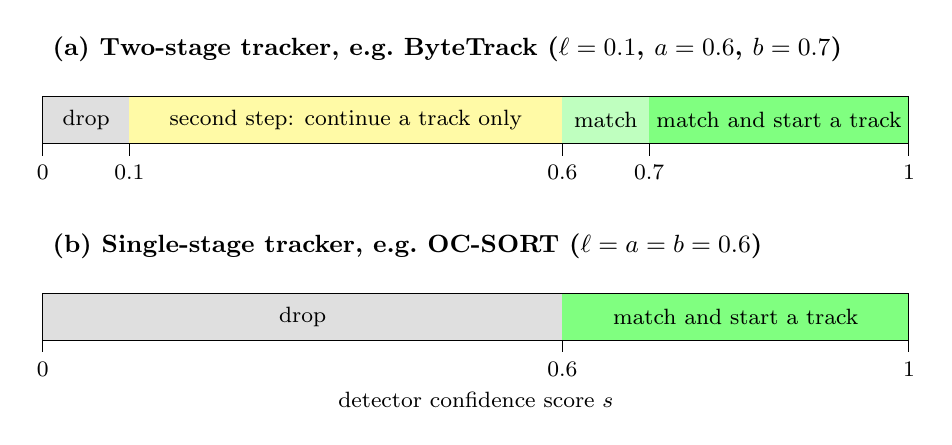
\begin{tikzpicture}[x=110mm, y=1mm, font=\small]
% two-stage tracker (ByteTrack, official setting): l = 0.1, a = 0.6, b = 0.7
\node[anchor=west, font=\small\bfseries] at (0,27) {(a) Two-stage tracker, e.g.\ ByteTrack ($\ell=0.1$, $a=0.6$, $b=0.7$)};
\fill[gray!25] (0,15) rectangle (0.1,21);
\fill[yellow!35] (0.1,15) rectangle (0.6,21);
\fill[green!25] (0.6,15) rectangle (0.7,21);
\fill[green!50] (0.7,15) rectangle (1,21);
\draw (0,15) rectangle (1,21);
\node[font=\footnotesize] at (0.05,18) {drop};
\node[font=\footnotesize] at (0.35,18) {second step: continue a track only};
\node[font=\footnotesize] at (0.65,18) {match};
\node[font=\footnotesize] at (0.85,18) {match and start a track};
\foreach \x/\l in {0/0, 0.1/0.1, 0.6/0.6, 0.7/0.7, 1/1} \draw (\x,15) -- (\x,13.5) node[below, font=\footnotesize] {\l};
% single-stage tracker (OC-SORT): l = a = b = 0.6
\node[anchor=west, font=\small\bfseries] at (0,2) {(b) Single-stage tracker, e.g.\ OC-SORT ($\ell=a=b=0.6$)};
\fill[gray!25] (0,-10) rectangle (0.6,-4);
\fill[green!50] (0.6,-10) rectangle (1,-4);
\draw (0,-10) rectangle (1,-4);
\node[font=\footnotesize] at (0.3,-7) {drop};
\node[font=\footnotesize] at (0.8,-7) {match and start a track};
\foreach \x/\l in {0/0, 0.6/0.6, 1/1} \draw (\x,-10) -- (\x,-11.5) node[below, font=\footnotesize] {\l};
\node[font=\footnotesize] at (0.5,-17.5) {detector confidence score $s$};
\end{tikzpicture}
\end{document}
